\documentclass{foi}
\usepackage[utf8]{inputenc}
\usepackage[croatian]{babel}
\usepackage{amsmath}
\usepackage{amsfonts}
\usepackage{amssymb}
\usepackage{lipsum}
\usepackage{float}
\usepackage[table]{xcolor}
\usepackage{threeparttable}
\usepackage{xcolor}
\usepackage{tabu}
\usepackage{graphicx}
\usepackage[export]{adjustbox}
\usepackage{enumitem}

\usepackage{pgfplots}
\pgfplotsset{compat=1.18}

\usepackage{chngcntr}
\counterwithout{equation}{chapter}

\usepackage{listings}
\lstset { %
    language=C++,
    backgroundcolor=\color{black!5}, % set backgroundcolor
    basicstyle=\footnotesize,% basic font setting
    numbers=left,
    stepnumber=1,
    showstringspaces=false,
    tabsize=1,
    breaklines=true,
    breakatwhitespace=false,
}

% \DeclareUnicodeCharacter{0140}{!!!!!}

\vrstaRada{\seminarski} % \zavrsni \diplomski
\title{Bloom filter}

\author{Zlatko Pračić}
\spolStudenta{\musko} % \zensko ili \musko
\mentor{Alen Lovrenčić}
\spolMentora{\musko} % \zensko ili \musko
\godina{2023}
\mjesec{lipanj}
\date{2023}
%\status{redoviti}
\indeks{00161450975}
\smjer{Razlikovna godina diplomskog studija - IPS} % (ili Poslovni sustavi, Ekonomika poduzetništva, Primjena informacijske tehnologije u poslovanju, Informacijsko i programsko inženjerstvo, Baze podataka i baze znanja, Organizacija poslovnih sustava, Informatika u obrazovanju)
\titulaProfesora{Prof. dr. sc. }

%\sazetak{Opsega od 100 do 300 riječi. Sažetak upućuje na temu rada, ukratko se iznosi čime se rad bavi, teorijsko-metodološka polazišta, glavne teze i smjer rada te zaključci.}

%\kljucneRijeci{riječ; riječ; ...riječ; Obuhvaća 7+/-2 ključna pojma koji su glavni predmet rasprave u radu.}

\begin{document}

\maketitle

\tableofcontents

\pagestyle{plain}
\chapter{Uvod}

\section{Predmet i cilj rada}
Predmet ovog seminarskog rada je apstraktni tip podataka (ATP) Bloom filter, koji je probabilistička struktura podataka korištena za učinkovitu provjeru prisustva elementa u skupu. Bloom filter nudi kompaktno rješenje na upit je li određeni element prisutan u skupu, bez potrebe za pohranjivanjem stvarnih elemenata skupa. To je ponekad vrlo korisna tehnika u situacijama kada su brzina i učinkovitost presudni, a ne postoji zahtjev za apsolutnom točnošću rezultata.

Cilj ovog rada je prikazati Bloom filter kao podatkovnu strukturu te istaći njegove karakteristike, prednosti i nedostatke. Kroz objašnjenje algoritma i matematičkih principa na kojima se zasniva, cilj je predočiti način na koji Bloom filter radi, kako se koristi i koje vrste problema može efikasno riješiti. Osim toga, kroz rad će se prikazati jedan od mogućih scenarija primjene Bloom filtra.

\section{Izvori podataka i metode prikupljanja}
Tijekom izrade seminarskog rada korišteni su različiti izvori informacija i to: relevantne knjige i znanstveni radovi koji opisuju općenito strukture podataka i algoritme te apstraktni tip podataka Bloom filter.

\section{Sadržaj i struktura rada}
Rad se sastoji od pet poglavlja od kojih je prvi uvod, a peti zaključak. Drugo poglavlje općenito opisuje Bloom filter, čemu isti služi i mogući način uporabe. U istom poglavlju je opisan način rada te vrste apstraktnog tipa podataka (ATP) i na koji način se određuju veličine vezane uz sam filter (veličina polja, broj unosa, broj funkcija sažimanja te kolika je mogućnost lažnih pozitivnih vrijednosti pri provjeri elemenata u polju). U trećem poglavlju se prikazuje kod sačinjen u C++ programskom jeziku pri čemu se pozornost daje načinu implementacije ATP-a i programu koji koristi ATP Bloom filter. U četvrtom se izračunala vremenska i amortizirana složenost Bloom filtra, a temeljem koda koji je dio rada.

\chapter{Opis ATP-a Bloom filter}

Bloom filter je vrsta podatkovne strukture nazvane po svom tvorcu, Burtonu Howardu Bloomu. Sličan je tablici sažetaka (eng. hash table), osim što umjesto pohranjivanja podataka, samo odgovara na upit je li podatak u skupu. Prednost Bloomovog filtra je što koristi manje memorije nego tablica sažetaka, no postoji kompromis između točnosti i iskorištenja memorije. Bloom filtri mogu proizvesti lažno pozitivne rezultate, a brisanje vrijednosti iz Bloom filtra nije izvedivo. Kako bi se dobio odnos između lažnih pozitivnih rezultata i prostora koji se zauzima postoji formula koja se može koristiti za izračunavanje količine memorije potrebne za održavanje stope lažno pozitivnih rezultata ispod određenog praga. Ista će se moći vidjeti dalje u radu \cite{la2021advanced}.

La Rocca u svojoj knjizi opisuje implementaciju Bloom filtera, koji se sastoji od polja m veličine i zbirke k funkcija sažimanja (eng. \textit{hash functions}). Svaki element polja početno je postavljen na 0, a svaka funkcija sažimanja vraća indeks između 0 i m-1. Kada se novi element doda filtru, indeksi niza se izračunavaju korištenjem funkcija sažimanja (ovisno o broju sažimanja koji se koristi) i postavljaju na 1. Da bi se pretražila stavka, izračunaju se sažimanja i ako su svi bitovi na tim lokacijama postavljeni na 1, smatra se da je unos u filtru (mora se paziti na lažne pozitivne rezultate) \cite{la2021advanced}.

\section{Namjena ATP Bloom filter}
Bloom filtar je sažeto probabilističko predstavljanje skupa podataka i koristi se za ispitivanje nalazi li se određena stavka u skupu ili ne. Osnovni Bloom filtar sastoji se od polja bitova i određenog broja funkcija sažimanja. Funkcije sažimanja koriste se za mapiranje svake stavke u jednoj od pozicija polja. Nakon sažimanja ulaznog elementa, vrijednost koja se dobije kao sažetak služi kao broj elementa polja koji se iz 0 mijenja u 1 (iz „false“ u „true“). Ta akcija se obavlja na isti način onoliko puta koliko se puta sažima sadržaj pa na primjer ako se koriste tri funkcije sažimanja onda se ista radnja provodi tri puta. S druge strane, postojanje se provjerava tako što se nakon sažimanja ulazne vrijednosti provjerava jesu li polja niza postavljena na nula ili jedan. Bloom filtar ima sljedeće prednosti: ima mali memorijski otisak, ima brzu i dosljednu brzinu upita i ažuriranja te ne daje lažno negativne rezultate i ima nisku stopu lažno pozitivnih rezultata, ali ta stopa se da konfigurirati na prihvatljivu razinu. Zbog ovih prednosti, Bloom filtar i njegove varijante naširoko se koriste u širokom rasponu područja pa su neka od područja gdje se Bloom filter koristi: sustavi u stvarnom vremenu, računalne arhitekture, neuronske mreže, IP pretraživanja, P2P mreže podatkovnih centara, računalstvo u oblaku  \cite{wu2021elastic}.

Međutim, Bloom filtar ima dva glavna nedostatka: unesene podatke nije moguće izbrisati niti je moguće listu proširiti. Konkretno, nakon što je stavka umetnuta u standardni Bloom filtar, stavka se ne može izravno izbrisati. Pored toga, nakon što je skup umetnut u Bloom filtar, nemoguće je konstruirati veći Bloom filtar koji predstavlja isti skup bez dodatnih informacija. Bez obzira na navedene nedostatke, Bloom filter je najbolji izbor u mnogim primjenama iako te aplikacije neizbježno pate od gore navedenih nedostataka pa se navedeni ATP koristi na primjer za:

\textbf{Crne liste} - Bloom filter se koristi za pohranjivanje crne liste za sprječavanje prijetnji kao što su DDoS napadi i razne verzije te vrste napada. Nedostatak ovog pristupa može biti mogućnost postavljanja upita za IP adresu koja je legalna te rezultat može biti lažno pozitivan i IP adresa će se smatrati zlonamjernom. Kako bi se riješio taj problem, postavlja se bijela lista za pohranu prijateljskih adresa.

\textbf{Traženje MAC adrese} - Svaki preklopnik (eng. \textit{switch}) ima tablicu MAC adresa. Tablica ima velik broj unosa i svaki se unos može smatrati parom ključ-vrijednost. Ključ je odredišna MAC adresa, a vrijednost je odlazni port. Jedan Bloom filtar izgrađen je za sve MAC adrese s istim odlaznim portom  \cite{wu2021elastic}.


\section{Problemski zadatak}
U svojoj knjizi La Rocca opisuje hipotetsku situaciju u kojoj je zaposleniku povjerena izgradnja nove značajke pri redizajnu usluge e-pošte. Pri tome jedna od novijih opcija bi bila da se prije dodavanja nove email adrese provjeri je li ona već na popisu postojećih adresa u adresaru. Resursi projekta su ograničeni, a zaposlenik ne može pozivati bazu podataka svaki put kada treba usporediti adresu e-pošte s popisom kontakata (želi se vidjeti nalazi li se adresa u adresaru). U knjizi autor preporučuje tehniku u kojoj se popis kontakata dobiva asinkrono i sprema u prostor za pohranu sesije, omogućujući zaposleniku da provjeri lokalnu kopiju podataka svaki put kada traži postojeće kontakte. Nakon što je lista pohranjena na lokalnom računalu, potrebno je provjeriti nalazi li se adresa u listi ili ne. Time se dolazi do problema rada s rječnikom, što je čest računalni problem traženja određenog unosa na popisu \cite{la2021advanced}.

Kako bi se traženo provelo na efikasan način postoji potreba za strukturom podataka koja može učinkovito upravljati operacijama poput preuzimanja, pohranjivanja i traženja kontakata. Obična polja nisu učinkovita za takve operacije jer im nedostaje metoda za brzo pronalaženje indeksa elementa ili određivanje je li element u polju. Autor predlaže asocijativno polje pošto isti ima izvornu metodu za učinkovit pristup pohranjenim unosima s pretraživanjem po vrijednosti. Redoslijed umetanja u asocijativno polje nije bitan i može pohranjivati parove (ključ, vrijednost). Korištenje apstrakcije rječnika omogućuje fokusiranje na zadatak rješavanja problema bez potrebe za rješavanjem detalja reprezentacije strukture podataka \cite{la2021advanced}.

Nadalje, autor raspravlja o asocijativnom polju, koji su zbirke parova (ključ, vrijednost) gdje se svaki ključ pojavljuje najviše jednom i svaka se vrijednost može dohvatiti izravno preko odgovarajućeg ključa i predlaže korištenje asocijativnog polja za pohranjivanje korisničkog adresara, koji se prima od poslužitelja kada se prijavi. Rječnik se čuva u memoriji i ažurira pozivima za umetanje i uklanjanje. Kada korisnik napiše e-poštu i unese primatelja, rječnik se provjerava je li kontakt u adresaru. Ako nije, pojavit će se skočni prozor s pitanjem želi li korisnik spremiti novi kontakt. Ovaj pristup minimizira HTTP pozive poslužitelju i čita iz baze podataka samo jednom pri pokretanju \cite{la2021advanced}.

\section{Načini moguće implementacije zadatka}

U nastavku autor govori o implementaciji asocijativnih polja u stvarnim sustavima. Ako je domena (skup mogućih ključeva) dovoljno mala, može se definirati ukupni poredak na ključevima i može se koristiti pravo polje, s nedostajućim vrijednostima postavljenim na \textit{null}. Međutim, u većini slučajeva, skup mogućih vrijednosti za ključeve je prevelik da bi se koristilo polje s elementom za svaku moguću vrijednost ključa, jer bi to zahtijevalo previše memorije. Autor je opisao četiri često korištene alternative za prevladavanje ovog problema s memorijom. Nakon opisa svih opcija bit će prikazana i tablica s vrijednostima vremena izvođenja operacija \cite{la2021advanced}:

\textbf{Nesortirano polje.}
Generalno za ovu vrstu polja autor kaže kako se u isto brzo umeće podatak, ali se jako sporo pretražuje i pronalazi. Tiskana knjiga bi mogla biti primjer gdje su riječi navedene redoslijedom kojim su ispisane. Ako je potrebno pronaći određenu riječ, kao što je na primjer "Bloom", mora se pretraživati knjiga riječ po riječ dok se ne pronađu sva pojavljivanja te riječi. Nerazvrstana polja ne zahtijevaju dodatni rad na stvaranju, a dodavanje novog unosa je jednostavno, ali pronalaženje određenih unosa može potrajati dugo \cite{la2021advanced}.

\textbf{Sortirano polje i binarno pretraživanje.}
Za ovu vrstu implementacije autor navodi kako je kod iste sporo umetanje podataka i brzo pretraživanje. Kod ove implementacije se koriste indeksi sortiranih popisa za učinkovito pretraživanje. Binarno pretraživanje može koristiti za traženje određene riječi na sortiranom popisu (kao na primjer telefonski imenik). Takva vrsta pretraživanja uključuje početak od otprilike polovice, provjeravanje nalazi li se riječ prije ili poslije tog mjesta. Ono što je specifično za ovu vrstu implementacije je da početno sortiranje i naknadno unošenje podataka (uz zahtjev da se uređenost zadrži) zahtjeva puno resursa \cite{la2021advanced}.

\textbf{Hash tablica.}
Hash tablice se koriste za implementaciju asocijativnih polja gdje moguće vrijednosti za pohranjivanje dolaze iz vrlo velikog skupa (na primjer, svi mogući nizovi ili svi cijeli brojevi), ali obično ih se treba pohraniti samo ograničen broj. Ako je to slučaj, tada se koristi funkcija sažimanja za mapiranje skupa mogućih vrijednosti (domena ili izvorni skup) u manji skup od M elemenata (kodomena ili ciljni skup). Uobičajeno se skup vrijednosti u domeni naziva ključevima, a vrijednosti u kodomeni indeksima od 0 do M-1. Budući da je ciljni skup funkcije sažimanja obično manji od izvornog skupa, doći će do sukoba: najmanje dvije vrijednosti bit će preslikane u isti indeks. Hash tablice koriste nekoliko strategija za rješavanje tog problema i to ulančavanje ili otvoreno adresiranje \cite{la2021advanced}.

\textbf{Binarno stablo.}
Sljedeća vrsta implementacije je binarno stablo. Ista koristi svojstva ukupnog uređenja u cilju osiguranja da se položaj ključa u stablu može odrediti gledanjem jedne staze od korijena do lista. Sve operacije na binarnom stablu zahtijevaju vrijeme proporcionalno visini stabla, što je $O(ln(n))$ za uravnoteženo binarno stablo. Iako je izvedba binarnog stabla na osnovnim operacijama sporija od hash tablica, ono ima prednost u pronalaženju prethodnika i sljedećeg ključa, te pronalaženju minimuma i maksimuma, pri čemu se sve te operacije izvode u $O(\ln(n))$ asimptotskom vremenu. Dodatno, binarno stablo može vratiti sve pohranjene ključeve, sortirane po ključu, u linearnom vremenu, dok hash tablice zahtijevaju sortiranje nakon dohvaćanja skupa ključeva.
\newpage
Tablica \ref{table:tablica1} prikazuje vremena izvođenja glavnih operacija na navedenim implementacijama rječnika \cite{la2021advanced}.

\begin{table}[H]
\centering
\def\arraystretch{1.4}
\caption{Složenost operacija na rječnicima za različite implementacije}
\begin{threeparttable}
\begin{tabular}{l|c|c|c|c}
\hline
\rowcolor[HTML]{416A85}
\color{white} Operacija & \color{white} Nesortirano polje & \color{white} Sortirano polje & \color{white} Binarno stablo & \color{white} Hash tablica\\ 
\hline 
Kreiranje strukture & $O(1)$ & $O(n*\log(n))$ & $O(n*\log(n))$ & $O(n)$ \\ 
\hline 
Traženje unosa & $O(n)$ & $O(\log(n))$ & $O(\log(n))$ & $O(n/M)$ \tnote{a} \\ 
\hline 
Unos novog podatka & $O(1)$ \tnote{a}& $O(n)$ & $O(\log(n))$ & $O(n/M)$ \tnote{a} \\ 
\hline 
Brisanje unosa & $O(1)$ & $O(n)$ & $O(\log(n))$ & $O(n/M)$ \tnote{a} \\ 
\hline 
Sortiranje & $O(n*\log(n))$ & $O(n)$ & $O(n)$ & $O(M+n*log(n))$ \\ 
\hline 
Min/Max & $O(n)$ & $O(1)$ & $O(1)$ \tnote{b} & $O(M+n)$\\ 
\hline
Sljedeći/Prethodni & $O(n)$ & $O(1)$ & $O(\log(n))$ & $O(M+n)$ \\ 
\hline
\end{tabular}
\begin{tablenotes}
     \item[a] \begin{small}Amortizirana vrijednost\end{small}
     \item[b] \begin{small}Odvojenim pohranjivanjem max/min i amortiziranjem vremena za njihovu zamjenu pri umetanju/brisanju\end{small}
   \end{tablenotes}
   \end{threeparttable}
\label{table:tablica1}
\end{table}

\textbf{Bloom filter.}
Za Bloom filter autor kaže kako je brz kao hash tablica, ali da pri tome štedi na memoriji računala. Postoje značajne razlike između hash tablica i Bloom filtara i one su:
\begin{itemize}
    \item Osnovni Bloom filtri ne pohranjuju podatke, oni samo odgovaraju na pitanje je li podatak u skupu?
    \item Zahtjevi Bloom filtra za memorijom su manji u usporedbi s hash tablicama; to je glavni razlog njihove upotrebe.
    \item Iako je negativan odgovor 100\% točan, može biti lažno pozitivnih odgovora.
    \item Nije moguće izbrisati vrijednost iz Bloomovog filtra \cite{la2021advanced}.
\end{itemize}

Postoji kompromis između točnosti Bloomovog filtra i memorije koju koristi. Što je manje memorije, vraća se više lažno pozitivnih rezultata. Međutim, postoji točna formula koja, s obzirom na broj vrijednosti koje se trebaju pohraniti, može izračunati količinu memorije potrebnu za održavanje stope lažno pozitivnih rezultata unutar određenog praga \cite{la2021advanced}.

\section{Kako radi Bloom filter}
Bloom filter se sastoji se od dva elementa: polje od $m$ elemenata i skup $k$ funkcija sažimanja. Polje od $m$ elemenata se inicijalno postavlja na 0. Svaka funkcija sažimanja daje indeks između $0$ i $m-1$. Korisniku je važna informacija kako ne postoji odnos 1-na-1 između elemenata polja i ključeva koji se dodaju Bloom filtru. Umjesto toga, koristi se $k$ bitova (i stoga $k$ elemenata polja) za pohranu svakog unosa za Bloom filtar. U ovom slučaju $k$ je ovdje obično mnogo manji od $m$. Potrebno je imati na umu da je $k$ konstanta koja se bira pri stvaranju strukture podataka, tako da svaki unos koji se dodaje pohranjen koristeći istu količinu memorije, točno $k$ bitova \cite{la2021advanced}.

To znači da se mogu dodati proizvoljno dugačka polja filtru koristeći stalnu količinu memorije. Kada se umetne novi ključ elementa u filtar, izračunava se $k$ indeksa za polje, danih vrijednostima $h_0$(ključ) do $h_{(k-1)}$(ključ) i ti se bitovi postavljaju na 1. Kada se traži unos, također treba izračunati $k$ sažimanja za njega kao što je opisano za umetanje, ali ovaj put se provjerava $k$ bitova na indeksima koje vraćaju funkcije sažimanja i vraća se $true$ akko su svi bitovi na tim pozicijama postavljeni na 1. Slika \ref{fig:vremena2} prikazuje obje operacije \cite{la2021advanced}.

\begin{figure}[H]
    \centering
    \includegraphics[width=0.9\textwidth, frame]{slike/input.png}
    \caption{Prikaz rada Bloom filtra \cite{la2021advanced}}
    \label{fig:vremena2}
\end{figure}

U nastavku je objašnjenje rada Bloom filtra prikazanog na Slici \ref{fig:vremena2}.
\begin{enumerate}[label=\Alph*)]
\item Na početku je filtar niz nula.
\item Pohrana stavki $x_i$ počinje tako što se svaki element sažima $k$ puta (u primjeru se vidi kako je $k=3$), pri čemu svakim sažimanjem indeksu pridružuje vrijednost 1. Kako je filterom određeno da će biti 3 funkcije sažimanja vrijednost $x_1$ mijenja vrijednost u polju na tri mjesta. Isto tako se može primijetiti da $x_1$ i $x_2$ imaju djelomično preklapanje (oba pokazuju na šesti element).
\item Kako bi se provjerilo je li element $y_i$ u skupu, isti se sažima k puta dobivajući pri tom isto toliko indeksa. Nakon toga se čitaju odgovarajući bitovi i akko su svi postavljeni na 1, vraćamo \textit{"true"}. Na Slici \ref{fig:vremena2} se vidi kako je element $y_1$ postavljen (međutim, ne može se isključiti mogućnost da filter vraća lažno pozitivan rezultat), dok element $y_2$ nije u skupu jer jedan od indeksa generiranih njegovim sažimanjem ima 0. Za taj element se može sa 100\% sigurnošću reći kako nije u polju \cite{la2021advanced}.
\end{enumerate}

U idealnom slučaju, filtru je potrebno $k$ različitih nezavisnih funkcija sažimanja kako bi se osiguralo da se indeksi ne dupliciraju za istu vrijednost. Iako je teško dizajnirati velik broj nezavisnih funkcija sažimanja, postoji nekoliko rješenja koje pružaju dobre aproksimacije. Jedno rješenje je korištenje parametarske funkcije sažimanja $H(i)$, koja generira $k$ funkcija sažimanja pozivanjem generatora H na različite vrijednosti. Drugo rješenje je korištenje jedne funkcije sažimanja $H$, ali inicijalizacija liste $L$ s $k$ slučajnih i jedinstvenih vrijednosti te stvaranje $k$ vrijednosti sažetka dodavanjem ili povezivanjem $L[i]$ s ključem. Treće rješenje je korištenje dvostrukog ili trostrukog sažimanja. U implementaciji se često koristi dvostruko sažimanje s dvije nezavisne funkcije sažimanja: \textit{Murmur hashing} i \textit{Fowler-Noll-Vo hashing} \cite{la2021advanced}.

\section{Provjera i unos podatka uz pomoć Bloom filtra}
U nastavku će se prikazati na koji način se provjerava postojanje neke vrijednosti uz pomoć Bloom filtra te način na koji se neka vrijednost unosi u isti.

\subsection{Provjera vrijednosti}

Kako se radi o hipotetskom zadatku provjere postojanja nečije e-mail adrese u imeniku, prvo će se prikazati provjera postojanja. Ta operacija se može opisati kroz sljedeće korake:

\begin{enumerate}[label=\Alph*)]

\item Počinje se s e-poštom koja se želi provjeriti nalazi li se u imeniku i to \texttt{duffy@acme.com}.

\item Ključ (e-pošta) se obrađuje kroz skup funkcija sažimanja. U konkretnom primjeru sa Slike \ref{fig:vremena3} koriste se tri funkcije sažimanja i to $H_0$, $H_1$ i $H_2$.

\item Svaka hash funkcija proizvodi indeks za polje s binarnim vrijednostima. Konkretno u ovom slučaju se radi o indeksima $ \left\langle 9, 6, 2 \right\rangle$.

\item Pristupa se elementima polja na tim indeksima.

\item Na indeksima 2 i 9 vrijednost je 0 (\textit{false}), a na indeksu 6 je vrijednost 1 (\textit{true}).

\item Kako svi elementi polja na traženim indeksima ne pokazuju vrijednost 1 (\textit{true}) to može značiti samo jedno, a to je da tražena e-mail adresa \texttt{duffy@acme.com} nije pohranjen u Bloom filtru i vraća se vrijednost (\textit{false}). Isti tijek koraka će se provesti i za e-mail adresu \texttt{roger@acme.com}. U tom slučaju su svi elementi polja na traženim indeksima postavljeni na 1 (\textit{true}) što znači da je e-mail adresa \texttt{roger@acme.com} možda pohranjena u Bloom filteru i to s određenim stupnjem pouzdanosti \cite{la2021advanced}.
\end{enumerate}

\begin{figure}[H]
    \centering
    \includegraphics[width=0.9\textwidth, frame]{slike/input_.png}
    \caption{Provjera prisutnosti podatka uz pomoć Bloom filtra \cite{la2021advanced}}
    \label{fig:vremena3}
\end{figure}

\subsection{Unos vrijednosti}

Na Slici \ref{fig:vremena4} se može vidjeti grafički prikaz rada Bloom filtra to jest konkretne operacije unošenja podatka u Bloom filter.

\begin{enumerate}[label=\Alph*)]

\item Počinje se s e-poštom koju se želi pohraniti, konkretno \texttt{duffy@acme.com}.

\item Ključ (e-pošta) obrađuje se kroz skup funkcija sažimanja: broj funkcija je postavljen $k=3$, pa će biti tri različite funkcije sažimanja, $H_0$, $H_1$ i $H_2$.

\item Svaka funkcija sažimanja proizvodi indeks za binarno polje. U ovom slučaju su tri indeksa $ \left\langle 9, 6, 2 \right\rangle$.

\item Pristupa se elementima binarnog polja kod tih indeksa. Na indeksima 2 i 9 je 0, a na indeksu 6 je 1.

\item Mijenjaju se samo bitovi koji su bili postavljeni na 0 (u ovom primjeru, one na indeksima 2 i 9). Nakon toga su svi dijelovi kojemu su sažetci \texttt{duffy@acme.com} postavljeni na 1, tako da će svako buduće pretraživanje vratiti \textit{"true"} \cite{la2021advanced}.

\end{enumerate}

\begin{figure}[H]
    \centering
    \includegraphics[width=0.9\textwidth, frame]{slike/input__.png}
    \caption{Unos vrijednosti uz pomoć Bloom filtra \cite{la2021advanced}}
    \label{fig:vremena4}
\end{figure}

\section{Izračun lažno pozitivne vjerojatnost Bloom filtra}

Lažno pozitivna stopa vjerojatnosti Bloomovog filtra može se izvesti na temelju pretpostavke kako je svaka pozicija niza odabrana s jednakom vjerojatnošću funkcijama sažimanja. Neka $m$ označava broj bitova u Bloom filteru. Prilikom umetanja elementa u filtar, vjerojatnost da određeni bit nije postavljen na jedinicu funkcijom sažimanja dana je s formulom \cite{tarkoma2011theory}:

\begin{equation}\label{prva_formula}
    1- \frac{1}{m}
\end{equation}

Uzimajući u obzir $k$ funkcija sažimanja, vjerojatnost da bilo koja od njih nije postavila određeni bit na jedan je:

\begin{equation}\label{druga_formula}
    \left( 1- \frac{1}{m} \right)^k
\end{equation}

Nakon umetanja $n$ elemenata u filtar, vjerojatnost da je dati bit još uvijek nula je:

\begin{equation}\label{treca_formula}
    \left( 1- \frac{1}{m} \right)^{kn}
\end{equation}

Posljedično, vjerojatnost da je bit jedan je:

\begin{equation}\label{cetvrta_formula}
    1-\left( 1- \frac{1}{m} \right)^{kn}
\end{equation}

Za test članstva elementa, ako su svi $k$ položaji niza izračunati funkcijama sažimanja postavljeni na jedan, Bloom filtar tvrdi da element pripada skupu. Vjerojatnost da se to dogodi kada element nije dio skupa aproksimira se kao:

\begin{equation}\label{peta_formula}
    \left( 1-\left( 1- \frac{1}{m} \right)^{kn}\right)^k \approx \left( 1- e^{-kn/m} \right)^k
\end{equation}

Autori rada napominju kako je $e^{-kn/m}$ vrlo bliska aproksimacija $ \left( 1- \frac{1}{m} \right)^{kn} $. Lažno pozitivna vjerojatnost se smanjuje kako se veličina Bloomovog filtra, $m$, povećava. Vjerojatnost raste s $n$ kako se dodaje više elemenata. Minimiziranjem se želi smanjiti vjerojatnost lažno pozitivnih rezultata $\left( 1- e^{-kn/m} \right)^k$ s obzirom na $k$. To se postiže uzimanjem derivacije i izjednačavanjem s nulom što daje optimalnu vrijednost $k$:

\begin{equation}\label{sesta_formula}
    k_{opt}=\frac{m}{n} \ln 2 \approx \frac{9m}{13n}
\end{equation}

To rezultira lažno pozitivnom vjerojatnošću od približno:

\begin{equation}\label{sedma_formula}
    \left( \frac{1}{2} \right)^k \approx 0.6185^{m/n}
\end{equation}

Upotrebom optimalnog broja hash funkcija $k_{opt}$ preko lažno pozitivne vjerojatnosti se može pisati i ograničiti kao:

\begin{equation}\label{osma_formula}
    \frac{m}{n} \eqslantgtr \frac{1}{ \ln 2}
\end{equation}

Da bi se održala fiksna lažno pozitivna vjerojatnost, duljina Bloomovog filtra mora rasti linearno s brojem umetnutih elemenata gdje je $p$ željena lažno pozitivna stopa:

\begin{equation}\label{deveta_formula}
    m=- \frac{n \ln p}{ \left( \ln 2 \right)^2  }
\end{equation}

Slika \ref*{fig:bloom-filters} prikazuje lažno pozitivnu stopu vjerojatnosti $p$ kao funkcija broja elemenata $n$ u filtru i filtar veličina $m$. Optimalan broj funkcija sažimanja $k = \frac{m}{n} \ln 2$ je pretpostavljen. Za izračun se koristila formula $\left( 1-\left( 1- \frac{1}{m} \right)^{kn}\right)^k$ \cite{tarkoma2011theory}.

\begin{figure}[H]
    \centering
    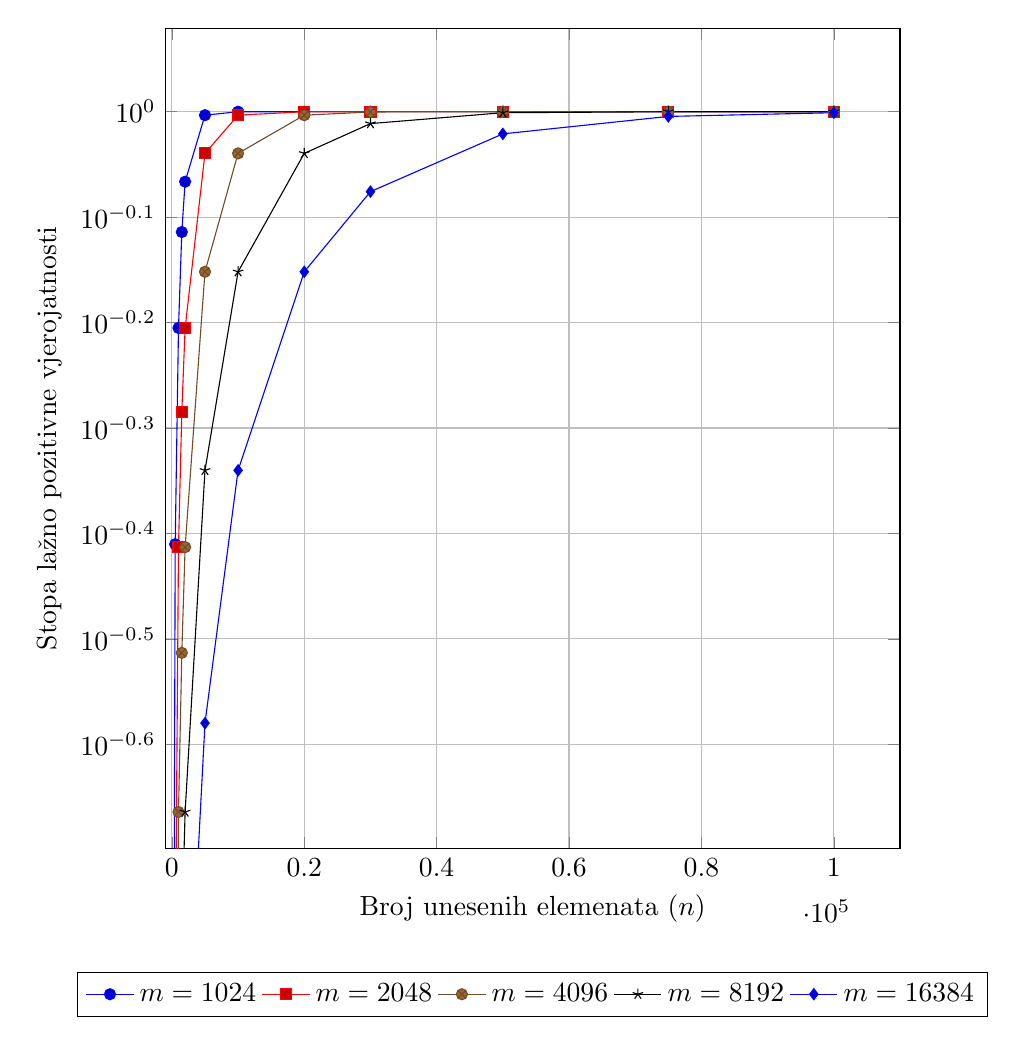
\begin{tikzpicture}
      \begin{semilogyaxis}[
        width=0.9\textwidth,
        height=12cm,
        xlabel={Broj unesenih elemenata ($n$)},
        ylabel={Stopa lažno pozitivne vjerojatnosti},
        grid=both,
        xmin=-1000, xmax=110000,  % Raspon domene na x-osi
        ymin=0.2, ymax=1.2,         % Raspon kodomene na y-osi
        legend style={at={(0.5,-0.15)},anchor=north},
        legend columns=-1
      ]
      
    % Vrijednosti Bloom filtera
    \addplot coordinates {
      (100,	0.00748482859684314)
      (200,	0.0865149039000977)
      (500,	0.388847279630001)
      (1000,	0.623576201943276)
      (1500,	0.76905125397066)
      (2000,	0.858305124256551)
      (5000,	0.992442374603577)
      (10000,	0.999942882298367)
      (20000,	0.999999996737568)
      (30000,	0.999999999999814)
      (50000,	1)
      (75000,	1)
      (100000,	1)
    };
    \addlegendentry{$m=1024$}
    
    \addplot coordinates {

    (100,	0.000119742944168711)
    (200,	0.0109427119202102)
    (500,	0.149299492217976)
    (1000,	0.386392924647923)
    (1500, 0.519342704972031)
    (2000,	0.623486357077871)
    (5000,	0.913013512679372)
    (10000,	0.992433351023618)
    (20000,	0.999942745823268)
    (30000,	0.999999566777742)
    (50000,	0.999999999975196)
    (75000,	1)
    (100000,	1)
    };
    \addlegendentry{$m=2048$}
    
    \addplot coordinates {
      (100,	0.000000982771)
      (200,	0.000991348167083419)
      (500,	0.0469354398598451)
      (1000,	0.216645885859494)
      (1500,	0.306674468914918)
      (2000,	0.386356331859144)
      (5000,	0.705021309507351)
      (10000,	0.912987572155242)
      (20000,	0.992428837400561)
      (30000,	0.999341214760615)
      (50000,	0.999995012229835)
      (75000,	0.999999988860655)
      (100000,	0.999999999975122)
    };
    \addlegendentry{$m=4096$}
    
    \addplot coordinates {
      (100,	0.000000005617)
      (200,	0.000074949409)
      (500,	0.013206712407425)
      (1000,	0.114920461221773)
      (1500,	0.16732897728102)
      (2000,	0.21663421003612)
      (5000,	0.456860354693513)
      (10000,	0.704999325696343)
      (20000,	0.912974602160388)
      (30000,	0.97432744895577)
      (50000,	0.997765836031818)
      (75000,	0.999894397897465)
      (100000,	0.999995008511363)
    };
    \addlegendentry{$m=8192$}
    
    \addplot coordinates {
      (100,	0.000000000027)
      (200,	0.000005158138)
      (500,	0.0035060121401616)
      (1000,	0.0592115878875208)
      (1500,	0.0874893555623855)
      (2000,	0.11491716363488)
      (5000,	0.263013050726083)
      (10000,	0.456850236599924)
      (20000,	0.704988334518442)
      (30000,	0.839764483693429)
      (50000,	0.952728653465101)
      (75000,	0.989722275779797)
      (100000,	0.997765419796778)
    };
    \addlegendentry{$m=16384$}
      
      \end{semilogyaxis}
    \end{tikzpicture}
    \caption{Stopa vjerojatnosti lažno pozitivnih vrijednosti za Bloom filter}
    \label{fig:bloom-filters}
  \end{figure}


\chapter{Implementacija Bloom filtra}

Bloom Filter podržava dvije osnovne operacije, a to su dodavanje i upit. Da bi se dodao (tj. umetnuo) element u filtar, element se prosljeđuje svakoj od k funkcija sažimanja i generira se k indeksa polja Bloom filtra. Odgovarajući bitovi u nizu tada se postavljaju na 1. Za provjeru prisutnosti elementa u skupu, element se prosljeđuje svakoj od funkcija sažimanja kako bi se dobili indeksi polja. Ako se utvrdi da bilo koji od bitova na tim pozicijama polja 0, tada se potvrđuje da element nije u skupu. Ako su svi bitovi na tim pozicijama postavljeni na 1, tada je element ili doista prisutan u skupu ili su bitovi postavljeni na 1 slučajno kada su drugi elementi umetnuti, što uzrokuje lažni pozitivni rezultat \cite{mei2013string}.

Nemoguće je ukloniti element iz Bloom filtra. To je zato što ako se odgovarajući bitovi elementa koji se uklanja vraćaju na 0, nema jamstva da ti bitovi ne nose informacije za druge elemente. Ako se jedan od tih bitova poništi, drugi element koji je slučajno kodiran na isti bit dat će negativan rezultat kada se upita, otuda izraz lažno negativan. Stoga bi jedini način uklanjanja elementa iz Bloom filtra bio rekonstruirati sam filtar bez neželjenog elementa. Rekonstrukcijom filtra lažno negativni rezultati bi bili eliminirani \cite{mei2013string}.

Stoga, sljedeće operacije će se obraditi u ovom seminarskom radu:
\begin{itemize}
  \item Konstruktor (ujedno i destruktor) $CreateBF()$
  \item Transformator $InsertBF(v)$
  \item Opservatori $IsElementBF(v)$
\end{itemize}

\section{ATP Bloom filter pomoću polja}

Na početku $bloom.h$ datoteke definiraju se osnovne postavke:

\begin{lstlisting}
#ifndef BLOOM
#define BLOOM 1000
#endif

#include <iostream>
#include <fstream>
#include <bitset>
#include <functional>

template <typename elementtype, int velicina_polja = BLOOM>

class BloomFilter ...
\end{lstlisting}

Ovaj dio koda koristi pretprocesorske direktive kako bi se definirala veličina polja u kojeg se smješta Bloom filter (konkretno nazvan "BLOOM"). U ovom primjeru se određuje polje veličine 1000 elemenata. Korisnik može u svom programu definirati isto, ali ako zaboravi ili ne definira tu vrijednost, ista je određena ovom linijom koda. Ako korisnik definira veličinu, tada se taj dio koda preskoči. Nakon toga se definira klasa $BloomFilter$.
\newpage
Potom se definira metoda $CreateBF()$ unutar klase $BloomFilter$:

\begin{lstlisting}
  void CreateBF()
  {
      filter.reset();
      std::ofstream izlazni_dokument(ime_dokumenta);
      if (izlazni_dokument.is_open())
      {
          izlazni_dokument << bloomfilter;
          std::cout << "Bloom filter je kreiran." << std::endl;
          izlazni_dokument.close();
      }
      else
      {
          std::cerr << "Nije moguce kreirati Bloom filter." << std::endl;
      }
  }
\end{lstlisting}

Ovom metodom se prvo resetiraju svi bitovi u filtru na vrijednost $0$ što osigurava da je filter prazan prije nego što se bilo koji element dodaje u njega. Nakon otvaranja datoteke koja je u ovom slučaju $bloom.txt$ (imenovana je u private dijelu u nastavku koda) i provjere uspješnosti otvaranja datoteke zapisuje se trenutno stanje u otvorenu datoteku i daje se poruka kako je filter kreiran. Na kraju se zatvara otvorena datoteku. Ako otvaranje datoteke nije uspjelo, ispisuje se poruka "Nije moguce kreirati Bloom filter". Iz ovog se može zaključiti kako metoda $CreateBF$ može služiti i za destrukciju samog polja i postavljanja na početnu vrijednost bez i jednog elementa u filtru.

Zatim se definira metoda $InsertBF()$ unutar klase $BloomFilter$:

\begin{lstlisting}
void InsertBF(const elementtype &vrijednost)
{
    std::fstream file(ime_dokumenta, std::ios::out | std::ios::in);
    if (file.is_open())
    {
        file >> bloomfilter;

        std::hash<elementtype> funkcija_sazimanja;
        std::size_t sazetak1=funkcija_sazimanja(vrijednost)%velicina_polja;
        std::size_t sazetak2=(funkcija_sazimanja(vrijednost)>>16)%velicina_polja;
        std::size_t sazetak3=(funkcija_sazimanja(vrijednost)>>32)%velicina_polja;

        bloomfilter.set(sazetak1, true);
        bloomfilter.set(sazetak2, true);
        bloomfilter.set(sazetak3, true);

        file.seekp(0);
        file << bloomfilter;
        file.close();

        std::cout << "Vrijednost '" << vrijednost << "' je dodana u Bloom filter." << std::endl;
    }
    else
    {
        std::cerr << "Nije moguce azurirati Bloom filter." << std::endl;
    }
}
\end{lstlisting}

Da bi se definirala metoda $InsertBF$ unutar klase $BloomFilter$ otvara se datoteka za čitanje i pisanje (datoteka je već kreirana). Provjerava se je li otvaranje datoteke uspjelo. Ako je otvaranje uspjelo, čita se trenutno stanje filtera iz datoteke. Nakon toga, stvara se objekt $funkcija\_sazimanja$ koji se koristi za generiranje sažetka vrijednosti. Tri različite vrijednosti sažetka se generiraju primjenom $funkcija\_sazimanja$. Ove vrijednosti sažetka se zatim koriste za postavljanje odgovarajućih bitova na $1$. Postavlja se pokazivač za pisanje na početak datoteke kako bi se filter zapisao na početak datoteke te se zapisuje trenutno stanje filtera u datoteku. Na kraju se zatvara otvorena datoteka. Kao izlaznu informaciju o provedenom, ispisuje se poruka kako je vrijednost dodana u Bloom filter. Ako otvaranje datoteke nije uspjelo, ispisuje se poruka da nije moguće ažurirati Bloom filter.

U nastavku se definira $IsElementBF()$ metoda unutar klase $BloomFilter$:

\begin{lstlisting}
bool IsElementBF(const elementtype &vrijednost)
{
    std::ifstream file(ime_dokumenta);
    if (file.is_open())
    {
        file >> bloomfilter;
        file.close();

        std::hash<elementtype> funkcija_sazimanja;
        std::size_t sazetak1=funkcija_sazimanja(vrijednost)%velicina_polja;
        std::size_t sazetak2=(funkcija_sazimanja(vrijednost)>>16)%velicina_polja;
        std::size_t sazetak3=(funkcija_sazimanja(vrijednost)>>32)%velicina_polja;

        return bloomfilter.test(sazetak1) && bloomfilter.test(sazetak2) && bloomfilter.test(sazetak3);
    }
    else
    {
        std::cerr << "Nije moguce otvoriti Bloom filter za provjeru." << std::endl;
        return false;
    }
}
\end{lstlisting}

Metoda $IsElementBF()$ otvara datoteku za čitanje i provjerava je li otvaranje datoteke uspjelo. Ako je otvaranje uspjelo, čita se trenutno stanje filtera iz datoteke. Zatim se stvara objekt $funkcija\_sazimanja$ koji se koristi za generiranje vrijednosti sažetka nakon čega se generiraju tri različite vrijednosti sažetka. Ove vrijednosti sažetka se zatim koriste za provjeru postavljenosti bitova. Nakon toga se zatvara otvorena datoteka. Na kraju, metoda vraća logički rezultat koji provjerava jesu li svi provjereni bitovi u filteru postavljeni na $1$. Ako jesu, vraća se $true$ inače se vraća $false$. Ako otvaranje datoteke nije uspjelo, ispisuje se poruka o nemogućnosti otvaranja filtra za provjeru.

Na kraju je deklariran privatan dio klase $BloomFilter$ i sadrži dvije privatne varijable.

\begin{lstlisting}
private:
  const std::string ime_dokumenta = "bloom.txt";
  std::bitset<velicina_polja> bloomfilter;
\end{lstlisting}

Deklarirano je ime datoteke  i to $bloom.txt$ te objekt tipa $bitset$ koji se koristi za pohranjivanje bitova Bloom filtera. Veličina bitseta je određena parametrom $velicina\_polja$, koji je postavljen na vrijednost $BLOOM$ ili $1000$ (prema definiciji iznad). Ovaj bitset predstavlja sam Bloom filter i koristi se za postavljanje ili provjeru postavljenosti pojedinih bitova u filteru. Ključna riječ $private$ označava da su ove varijable privatne, što znači da im se može pristupiti samo unutar klase $BloomFilter$ i nisu dostupne izvan nje. Takav način rada osigurava enkapsulaciju, ograničavajući izravan pristup tim varijablama izvan klase.

\section{Korištenje ATP Bloom filter}
U nastavku će se opisati program koji koristi ATP Bloom filter. Datoteka je nazvana $bloom.cpp$ i ista u svojim prvim redovima započinje uključivanjem potrebne biblioteke i $bloom.h$ datoteke. Deklariraju se tipovi podataka i konstanta $velicina\_polja$, koja predstavlja veličinu Bloom filtera. Da se veličina filtra nije odredila u korisničkom programu, ista bi ipak bila određena pošto se veličina deklarira i u $bloom.h$ datoteci te ako nije deklarirano ranije, bilo bi deklarirano kroz $bloom.h$ datoteku.

\begin{lstlisting}
#include <iostream>
#include "bloom.h"
  
typedef std::string elementtype;
  
const int velicina_polja = BLOOM;
BloomFilter<elementtype, velicina_polja> bloomFilter;
\end{lstlisting}

U funkciji $main()$ se koristi beskonačna petlja $while(true)$ kako bi se omogućilo korisniku da izvršava različite operacije sve dok ne odabere izlazak iz programa. Unutar petlje se ispisuje izbornik s različitim opcijama za manipulaciju Bloom filtrom. Kada korisnik odabere neku operaciju, unosi se odgovarajući broj izbornika (varijabla izbor) putem standardnog ulaza. Zatim se koristi $switch$ izraz za odabir odgovarajuće akcije na temelju unesenog broja.

Ako je izbor 1, poziva se metoda $CreateBF()$ na $bloomFilter$ objektu, koja stvara novi Bloom filter. Kod izbora broja 2 korisnika se traži unos vrijednosti, a zatim se poziva metoda $InsertBF()$ na $bloomFilter$ objektu, koja dodaje vrijednost u Bloom filter. Nakon izbora 3, korisniku se također traži unos vrijednosti, a zatim se poziva metoda $IsElementBF()$ na $bloomFilter$ objektu. Metoda provjerava je li vrijednost prisutna u Bloom filtru i vraća bool vrijednost ($true$ ako je vjerojatno prisutna, $false$ ako nije). Rezultat se ispisuje na standardnom izlazu. Po izboru broja 4, ispisuje se poruka o izlasku iz programa i petlja se prekida.

Ako korisnik unese neispravan broj (izbor koji nije 1, 2, 3 ili 4), ispisuje se poruka o neispravnom unosu i petlja se nastavlja. Nakon svake izvršene operacije, ispisuje se prazna linija radi razdvajanja ispisnih redaka. Kod završava s izrazom $return 0$, što označava uspješan završetak programa.

\begin{lstlisting}
int main()
{
    int izbor;
    while (true)
    {
        std::cout << "       Bloom filter - Izbornik       " << std::endl;
        std::cout << "-------------------------------------" << std::endl;
        std::cout << "1. Stvori Bloom filter               " << std::endl;
        std::cout << "2. Dodaj vrijednost u Bloom filter   " << std::endl;
        std::cout << "3. Provjeri vrijednost u Bloom filtru" << std::endl;
        std::cout << "4. Izlazak iz programa               " << std::endl;
        std::cout << "-------------------------------------" << std::endl;
        std::cout << "Unesi broj zeljene operacije: ";
        std::cin >> izbor;

        switch (izbor)
        {
        case 1:
            bloomFilter.CreateBF();
            break;
        case 2:
        {
            elementtype vrijednost;
            std::cout << "Unesi vrijednost: ";
            std::cin >> vrijednost;
            bloomFilter.InsertBF(vrijednost);
            break;
        }
        case 3:
        {
            elementtype vrijednost;
            std::cout << "Unesi vrijednost: ";
            std::cin >> vrijednost;
            bool exists = bloomFilter.IsElementBF(vrijednost);
            std::cout << "Vrijednost '" << vrijednost << (exists ? "' je mozda u" : "' nije u") << " Bloom filtru." << std::endl;
            break;
        }
        case 4:
            std::cout << "Izlazak iz programa" << std::endl;
            return 0;
        default:
            std::cout << "Neispravan unos. Pokusajte opet." << std::endl;
        }
        std::cout << std::endl;
    }
    return 0;
}
\end{lstlisting}

\chapter{Izračun složenosti i amortizirane složenosti}

Vremenska složenost algoritma odnosi se na procjenu koliko vremena je potrebno za izvršavanje algoritma u ovisnosti o veličini ulaza. Obično se izražava kroz notaciju $Big O$, koja pruža gornju granicu rasta vremena izvršavanja algoritma s povećanjem ulaza. Vremenska složenost je ključna za razumijevanje performansi algoritma i donošenje odluka o odabiru najboljeg algoritma za određeni problem \cite{levitin2014introduction}.

Amortizirana složenost je koncept koji se koristi za analizu algoritama koji povremeno izvršavaju operacije s velikom složenošću, ali se u prosjeku izvršavaju brzo. Ova analiza uzima u obzir ukupno vrijeme izvršavanja niza operacija umjesto samo pojedinačnih operacija. To omogućuje da se visoka složenost pojedinačnih operacija "amortizira" kroz vrijeme u kojem se izvršavaju brze operacije \cite{levitin2014introduction}.

\section{Vremenska složenost Bloom filtra}

Prvo će se prikazati vremenska složenost (za najgori slučaj) metode $CreateBF$.

\begin{lstlisting}
    void CreateBF()
    {
        bloomfilter.reset();                                        // O(c1)
        std::ofstream izlazni_dokument(ime_dokumenta);              // O(c2)
        if (izlazni_dokument.is_open())                             // O(c3)
        {
            izlazni_dokument << bloomfilter;                        // O(c4)
            std::cout << "Bloom filter je kreiran." << std::endl;   // O(b1)
            izlazni_dokument.close();                               // O(c5)
        }
        else
        {
            std::cerr << "Nije moguce kreirati Bloom filter." << std::endl;                                                     // O(b2)
        }
    }
\end{lstlisting}

Kako se radi o jednostavnoj operaciji inicijalizacije polja s unaprijed određenim brojem elemenata koji se postavljaju na vrijednost $0$ vremenska kompleksnost je (ako je $c_6=max \left\{ b_1, b_2 \right\}$):

\begin{equation*}
    \begin{aligned}
    T^{CreateBF}_{max} & \leq c_1 + c_2 + c_3 + c_4 + c_5 + c_6\\
    & =  d_1 \\
    \end{aligned}
\end{equation*}

Stoga, za operaciju kreiranja Bloom filtra se može reći kako iznosi $$ T^{CreateBF}_{max} \left( n \right) = O \left( 1 \right)$$
\newpage
\begin{lstlisting}
    void InsertBF(const elementtype &vrijednost)
{
    std::fstream file(ime_dokumenta, std::ios::out | std::ios::in);         // O(c1)
    if (file.is_open())                                                     // O(c2)
    {
    file >> bloomfilter;                                                    // O(c3)

    std::hash<elementtype> funkcija_sazimanja;                              // O(c4)
    std::size_t sazetak1=funkcija_sazimanja(vrijednost)%velicina_polja;     // O(c5)
    std::size_t sazetak2=(funkcija_sazimanja(vrijednost)>>16)%velicina_polja// O(c6)
    std::size_t sazetak3=(funkcija_sazimanja(vrijednost)>>32)%velicina_polja// O(c7)

    filter.set(sazetak1, true);                                             // O(c8)
    filter.set(sazetak2, true);                                             // O(c9)
    filter.set(sazetak3, true);                                            // O(c10)

    file.seekp(0);                                                         // O(c11)
    file << bloomfilter;                                                   // O(c12)
    file.close();                                                          // O(c13)

      std::cout << "Vrijednost '" << vrijednost << "' je dodana u Bloom filter." << std::endl;                                                       // O(b1)
    }
    else
    {
        std::cerr << "Nije moguce azurirati Bloom filter." << std::endl;   // O(b2)
    }
}
\end{lstlisting}

Operacija umetanja vrijednosti u polje ovisi o broju funkcija sažimanja koji je unaprijed određen. Vremenska kompleksnost je (ako je $c_{14}=max \left\{ b_1, b_2 \right\}$):

\begin{equation*}
    \begin{aligned}
    T^{InsertBF}_{max} & \leq c_1 + c_2 + c_3 + c_4 + c_5 + c_6 + c_7 + c_8 + c_9 + c_{10} + c_{11} + c_{12} + c_{13} + c_{14}\\
    & =  d_1 \\
    \end{aligned}
\end{equation*}

Stoga, za operaciju umetanja vrijednost u Bloom filtar se može reći kako iznosi $$ T^{InsertBF}_{max} \left( k \right) = O \left( 1 \right)$$

Ostalo je još za odrediti složenost provjere operacije kojom se provjerava je li uneseni element u Bloom filtru.

\begin{lstlisting}
    bool IsElementBF(const elementtype &vrijednost)
    {
        std::ifstream file(ime_dokumenta);                                  // O(c1)
        if (file.is_open())                                                 // O(c2)
        {
            file >> bloomfilter;                                            // O(c3)
            file.close();                                                   // O(c4)    
            std::hash<elementtype> funkcija_sazimanja;                      // O(c5)
    std::size_t sazetak1=funkcija_sazimanja(vrijednost)%velicina_polja;     // O(c6)
    std::size_t sazetak2=(funkcija_sazimanja(vrijednost)>>16)%velicina_polja// O(c7)
    std::size_t sazetak3=(funkcija_sazimanja(vrijednost)>>32)%velicina_polja// O(c8)
    
    return bloomfilter.test(sazetak1) && bloomfilter.test(sazetak2) && bloomfilter.test(sazetak3);                                                     // O(b1)
    }
    else
    {
    std::cerr <<"Nije moguce otvoriti Bloom filter za provjeru."<<std::endl;// O(b2)
    return false;                                                           // O(b3)
    }
}
\end{lstlisting}

Operacija provjere vrijednosti, slično operaciji umetanja vrijednosti u polje, ovisi o broju funkcija sažimanja. S unaprijed određenim brojem funkcija (u ovom slučaju 3) sažimanja vremenska kompleksnost je (ako je $c_9 =max \left\{ b_1, b_2 + b_3 \right\}$):

\begin{equation*}
    \begin{aligned}
    T^{IsElementBF}_{max} & \leq c_1 + c_2 + c_3 + c_4 + c_5 + c_6 + c_7 + c_8 + c_9\\
    & =  d_1 \\
    \end{aligned}
\end{equation*}

Stoga, za operaciju provjere vrijednosti u Bloom filtar se može reći kako je $$ T^{IsElementBF}_{max} \left( k \right) = O \left( 1 \right)$$

\section{Amortizirana složenost Bloom filtra}

Nakon izračuna vremenske složenosti Bloom filtra može se pristupiti izračunu amortizirane složenosti. Koristit će se metoda energetskih potencijala. Izračunat će se vrijednosti za operacije umetanja $InsertBF$ i provjere $IsElementBF$ pošto Bloom filter nema operaciju brisanja vrijednosti. Stvarne cijene operacija su $1$ i to je prikazano u Tablici \ref{table:tablica2}.

\begin{table}[H]
    \centering
    \def\arraystretch{1.4}
    \caption{Stvarne cijene operacija}
    \begin{tabular}{l|c}
    \hline
    \rowcolor[HTML]{416A85}
    \color{white} Operacija & \color{white} Cijena \\ 
    \hline 
    $InsertBF$ & $1$ \\
    \hline 
    $IsElementBF$ & $1$ \\
    \hline
    \end{tabular}
    \label{table:tablica2}
    \end{table}

Potom se može prijeći na izračun amortizirane vrijednosti. Samo operacija $InsertBF$ se povećava potencijal strukture podataka za $1$ tj. $ \Phi \left(D_i\right) = \Phi \left(D_{i-1}\right) + 1$ odnosno $ \Phi \left(D_i\right) - \Phi \left(D_{i-1}\right) = 1 $. Stoga je

\begin{equation*}
    \begin{aligned}
    \hat{c_i} \left(InsertBF\right) & = c \left(InsertBF\right) + 1\\
    & =  1 + 1 = 2 \\
    \end{aligned}
\end{equation*}

Iz istog proizilazi Tablica \ref{table:tablica3} :

\begin{table}[H]
    \centering
    \def\arraystretch{1.4}
    \caption{Amortizirane cijene operacija}
    \begin{tabular}{l|c}
    \hline
    \rowcolor[HTML]{416A85}
    \color{white} Operacija & \color{white} Cijena \\ 
    \hline 
    $InsertBF$ & $2$ \\
    \hline 
    $IsElementBF$ & $1$ \\
    \hline
    \end{tabular}
    \label{table:tablica3}
    \end{table}

Najgori slučaj je kada se izvede $N$ uzastopnih operacija $InsertBF$ i tada je

\begin{equation*}
    \begin{aligned}
    \sum_{i=1}^{N} c_i \left(O_i\right) & \leq \sum_{i=1}^{N} \hat{c_i} \left(O_i\right) \\
    & \leq  \sum_{i=1}^{N} \hat{c_i} \left( InsertBF \right) \\
    & = \sum_{i=1}^{N} 2 \\
    & = 2N
    \end{aligned}
\end{equation*}

Pa je:

$$ T^{BloomFilter} \left( N \right) = O \left( N \right)$$

\chapter{Zaključak}

Ovaj rad je pružio pregled Bloom filtera kao probabilističke strukture podataka za efikasnu provjeru prisustva elemenata u skupu. Prikazani su osnovni principi Bloom filtra, njegova implementaciju i karakteristike. Takođe su razmotrene prednosti i nedostaci ove strukture podataka, kao i neke od njegovih primjena u stvarnim situacijama.

Bloom filter je posebno koristan u situacijama gdje je brzina ključna, a mala vjerojatnost greške pri dobijanju lažno pozitivnih rezultata je prihvatljiva. On pruža kompaktno rješenje za provjeru prisustva elemenata u velikim skupovima podataka bez potrebe za čuvanjem samih elemenata. Međutim, mora se uzeti u obzir da Bloom filter može dati lažno pozitivne rezultate, ali nikada lažno negativne.

Iako Bloom filter ima svoje prednosti, kao što su niski memorijski zahtjevi i brze operacije provjere prisustva, treba biti oprezan prilikom odabira ove strukture podataka. Njegova efikasnost ovisi od odgovarajućeg odabira parametara, poput veličine filtera i broja funkcija sažimanja te od pravilne procjene potreba za točnošću rezultata. U nekim slučajevima, gdje je potrebna apsolutna točnost, bilo bi potrebno razmotriti alternative.

\listoffigures
\addcontentsline{toc}{chapter}{Popis slika}
 
\listoftables
\addcontentsline{toc}{chapter}{Popis popis tablica}
  
\printbibliography[title=Popis literature]
\addcontentsline{toc}{chapter}{Popis literature}

\end{document}